\chapter{Giovedì 04/03/2021 e Venerdì 05/03/2021}
%\section{Spazio di memoria, dimensionamento della memoria, formato degli indirizzi}
\section{Unità di misura della memoria} Dato un numero di bit, vogliamo indicare la dimensione dell'area di memoria con le apposite unità di misura. Osserviamo le potenze
\begin{align*}2^2=4&&2^3=8&&2^4=16&&2^5=32&&2^6=64&&2^7=128&&2^8=256&&2^9=512&&\boxed{2^{10}=1024}\end{align*}
A questo punto i dubbi ci vengono. Noi informatici abbiamo sempre abusato di queste lettere....
\begin{align*}
	2^{10}\simeq 1000 &\longrightarrow K&2^{20}\simeq 1000000 &\longrightarrow M\\
	2^{30}\simeq \dots &\longrightarrow G&2^{40}\simeq \dots &\longrightarrow T
\end{align*}
Cerchiamo di risolvere la confusione con la seguente tabella\begin{center}\begin{tabular}{ |l|c|l|l|c|l|} \hline\multicolumn{3}{|c|}{\textbf{Misure binarie}} & \multicolumn{3}{c|}{\textbf{Misure decimali}} \\\hline\textbf{Nome} & \textbf{Fattore} & \textbf{Valore in byte} & \textbf{Nome} & \textbf{Fattore} & \textbf{Valore in byte}\\\hline
		kibibyte (KiB) & $2^{10}$ & 1,024 & kilobyte (KB) & ${10}^3$ & 1,000\\ 
		\hline
		mebibyte (MiB) & $2^{20}$ & 1,048,576 & megabyte (MB) & ${10}^6$  & 1,000,000\\ 
		\hline
		gibibyte (GiB) & $2^{30}$ & 1,073,741,824 & gigabyte (GB) & ${10}^9$  & 1,000,000,000\\ 
		\hline
		tebibyte (TiB) & $2^{40}$ & 1,099,511,627,776 & terabyte (TB) & ${10}^{12}$  & 1,000,000,000,000\\ 
		\hline
	\end{tabular}
\end{center}

\noindent Abbiamo introdotto delle nuove unità di misura. Quelle "tradizionali" a cui siamo abituati sono \emph{misure decimali}, mentre quelle nuove sono \emph{misure binarie}. 
\begin{align*} 
	1\,\text{KB}&=1000\,\text{byte}&1\,\text{KiB}&=1024\,\text{byte}&\Delta&=24\,\text{byte}\\
	2\,\text{KB}&=2*1000=2000\,\text{byte}&2\,\text{KiB}&=2*1024=2048\,\text{byte}&\Delta&=48\,\text{byte}\\
	3\,\text{KB}&=3*1000=3000\,\text{byte}&3\,\text{KiB}&=3*1024=3072\,\text{byte}&\Delta&=72\,\text{byte}\\
	&=\dots&&=\dots&&=\dots\\
	N\,\text{KB}&=N*1000=N*{10}^3&N\,\text{KiB}&=N*1024=N*{10}^3+N*24&\Delta&=N*24\,\text{byte}
\end{align*}
Risulta facile capire che più le dimensioni aumentano più le misure binarie si discostano da quelle decimali.

\paragraph{Quanto spazio ho con 48 bit?} $2^{48}=2^{40} \cdot 2^{8}= 256\,\text{TiB}$
\paragraph{Quanto spazio ho con 57 bit?} $2^{57}=2^{50} \cdot 2^{7}= 128\,\text{PiB}$

\section{Spazio di memoria non completo e "buco"} Lo spazio di memoria non è completo: non tutti i 64bit che compongono un indirizzo sono implementati. La AMD si è riservata di poterne aggiungere in futuro. Lo ha già fatto: i primi processori avevano solo 48 bit significativi, adesso i bit significativi sono 57. Bit in più comportano complicazioni in più, soprattutto costo maggiore nell'utilizzo.
\paragraph{Formato degli indirizzi} \[\boxed{\text{I bit non utilizzati devono essere uguali al bit più significativo tra quelli utilizzati.}}\]Gli indirizzi che rispettano il formato sono detti in \textbf{forma canonica}. All'interno del processore esiste un meccanismo di protezione che impedisce al processore di andare avanti se l'indirizzo posto non rispetta il formato. La AMD ha adottato questo meccanismo remore dell'esperienza della IBM. Questa, quando ha cercato di implementare indirizzi più grandi, ha avuto problemi: molti programmi hanno smesso di funzionare perché utilizzavano i fili di indirizzo non implementati per altri scopi.

\paragraph{Conseguenza} All'interno dello spazio di memoria abbiamo una sorta di buco, che va dall'ultimo indirizzo avente tutti e 7 i bit più significativi uguali a $0$ al primo indirizzo avente tutti e 7 i bit più significativi uguali ad $1$.

\section{Esempio di programma Assembler}
\paragraph{Esami su Linux} Gli esami saranno svolti su macchina virtuale con Debian. Non è necessario avere grande dimestichezza verso questo sistema operativo.
\paragraph{Funzionamento}
\begin{itemize}
	\item Produciamo un file editor.s
	\item L'assemblatore produce, a partire dal file precedente, un file oggetto .o. I file oggetto sono semplici dati, nulla di eseguibile. 
	\item Il collegatore unisce questo file oggetto con altri files oggetto (librerie) e crea un eseguibile. 
\end{itemize}
Contrariamente al Manchester Baby \textbf{stiamo creando programmi utilizzando altri programmi}. Non è necessario che i files oggetto siano presenti sul dispositivo dove avvieremo l'eseguibile: quando acquistiamo un programma abbiamo solo ciò che serve per eseguire il programma, non gli elementi utilizzati per creare il programma.
\paragraph{Come creiamo programmi in una macchina nuova che non ha assemblatore?} Creiamo l'assemblatore e il collegatore su una macchina già esistente: il risultato gira sulla macchina vecchia, ma funziona anche sulla macchina nuova. Otteniamo l'eseguibile sulla macchina vecchia e lo poniamo nella macchina nuova. 
\paragraph{In che linguaggio è scritto il compilatore per il C?} In C. Come è possibile? 
\begin{itemize}
	\item I compilatori moderni sono compilati da versioni precedenti.
	\item La prima versione del compilatori in C è scritta in un altro linguaggio.
	\item I primi compilatori, successivamente, sono stati scritti in linguaggio assembler.
	\item I primi assemblatori sono stati scritti in linguaggio macchina.
\end{itemize}
\paragraph{Assemblatore} L'assemblatore traduce dal linguaggio assembler al linguaggio macchina. Precisamente, lo vediamo dal nome, l'assemblatore assembla il contenuto della memoria (programmare significa indicare il contenuto iniziale della memoria). Fa ciò che noi abbiamo fatto a mano per scrivere un programma nel Manchester Baby.
\paragraph{perché separare assemblatore e collegatore?} Conviene scrivere questi pezzi di memoria senza decidere dall'inizio dove dovranno essere caricati. Scrive le cose, ma rimanda la decisione: questo perché vuole scrivere tanti pezzi (quando scrive un pezzo non sa riguardo gli altri). 

\paragraph{Codice}
\small
\begin{verbatim}
	.data
	num1:
	.quad 0x1122334455667788
	num2:
	.quad 0x9900aabbccddeeff
	risu:
	.quad -1
	
	.text
	.global _start
	_start:
	movabs num1, %rax
	mov %rax, %rbx
	movabs num2, %rax
	add %rbx, %rax
	movabs %rax, risu
	
	# uscita
	mov $0, %rbx   
	mov $1, %rax
	int $0x80
\end{verbatim}
\normalsize
\paragraph{Raggiungiamo il terminale}
\begin{center}
	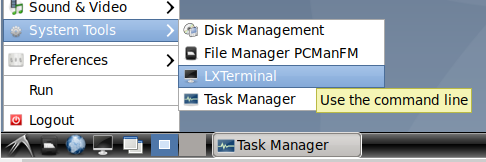
\includegraphics{img/138.PNG}
\end{center}
\paragraph{Comandi eseguiti} In una riga pongo prima il comando, e poi gli argomenti
\begin{itemize}
	\item \begin{verbatim}ls\end{verbatim}
	carico la lista dei files presenti nella directory
	\begin{center}
		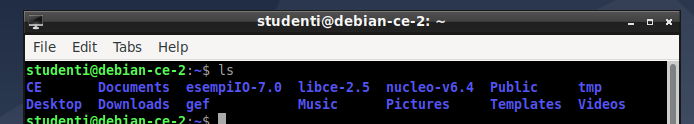
\includegraphics[scale=.8]{img/135.PNG}
	\end{center}
	se non sono presenti files/cartelle non restituisce nulla.
	\item \begin{verbatim}cd nome_cartella\end{verbatim}
	accedo a una directory
	\begin{center}
		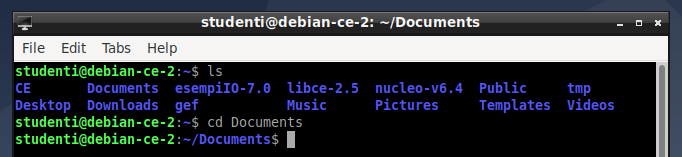
\includegraphics[scale=.8]{img/136.PNG}
	\end{center}
	Nel caso in cui la directory non esista viene restituito l'errore \emph{No such file or directory}. Per tornare indietro di una directory basta porre due punti come nome della cartella
	\begin{center}
		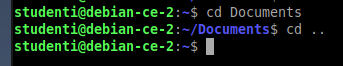
\includegraphics[scale=.9]{img/137.PNG}
	\end{center}
	\item \begin{verbatim}mkdir nome_cartella\end{verbatim}
	creo una cartella col nome indicato.
	\item \begin{verbatim}vi sum.s\end{verbatim}
	carico l'editor di modifica per il file \emph{sum.s}. 
	\begin{center}
		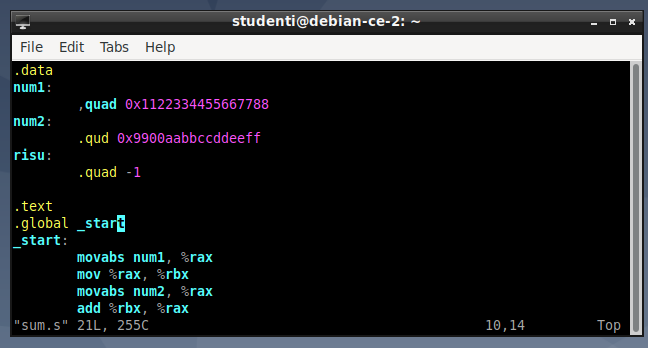
\includegraphics[scale=.8]{img/139.PNG}
	\end{center}Se il file esiste viene caricato l'editor di modifica per quel file, se non esiste viene caricato l'editor lo stesso e in caso di salvataggio viene creato. Si tenga conto che al caricamento dell'editor entriamo in modalità comando.
	\begin{itemize}
		\item Per entrare in modalità modifica digitare la seguente lettera
		\begin{verbatim}i\end{verbatim}
		che permette di iniziare la modifica a partire dal carattere dove si trova il cursore del terminale (altre lettere permettono di entrare in modalità modifica, la differenza sta nel punto da dove inizieremo a modificare).
		\item Per ritornare alla modalità comando basta utilizzare il tasto \emph{ESC}.
		\item Per annullare modifiche precedenti digitare la seguente lettera
		\begin{verbatim}u\end{verbatim}
		\item Per chiudere l'editor e salvare le modifiche fatte utilizzare il seguente comando
		\begin{verbatim}:wq\end{verbatim}
		se invece non vogliamo salvare le modifiche
		\begin{verbatim}:q\end{verbatim}
	\end{itemize}
	\item \begin{verbatim}as -o sum.o sum.s\end{verbatim}
	indico che voglio assemblare il programma. Tradizione UNIX è l'assenza di messaggi se tutto va bene. Indico col secondo parametro il nome da dare all'output (\emph{sum.o}), mentre col terzo indico il file Assembler che voglio assemblare (\emph{sum.s}). 
	\item \begin{verbatim}objdump -d sum.o\end{verbatim}
	esamino il contenuto del file oggetto indicato. Con l'opzione d chiedo il \emph{disassembly}, cioè chiedo di rigenerare il file assembler originario partendo dal binario. \begin{center}
		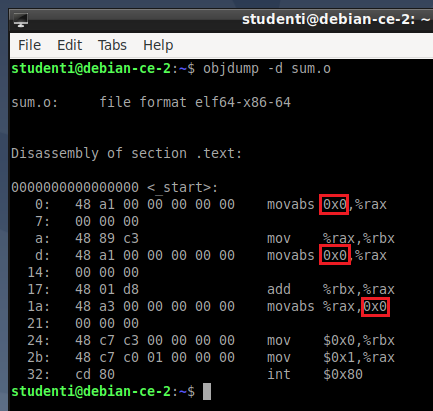
\includegraphics{img/140.PNG}
	\end{center}
	\begin{itemize}
		\item Il formato del file disassemblato è: \emph{file format elf64-x86-6}
		\item Si osservi che l'assemblatore non sa dove stanno \emph{$\_$start}, \emph{num1}, \emph{num2} e \emph{risu}.
		\begin{itemize}
			\item Nella prima \emph{movabs} non sappiamo dove finirà \emph{num1} (e non può fare ipotesi sull'offset, visto che le parti data e le parti text saranno unificate in presenza di più files). L'istruzione è identificata dal byte \emph{a1}, che rappresenta l'istruzione e il passaggio da un indirizzo al registro RAX. Sono riservati 8 byte per l'indirizzo.
			\item La prima \emph{mov} ha solo operandi registro, è molto più compatta. La codifica identifica la \emph{mov} e il passaggio da registro RAX a registro RBX (\emph{89 c3}).
			\item Il numero 48, posto all'inizio di alcune istruzioni, è il prefisso introdotto dalla AMD per le istruzioni che devono usare operandi a 64 bit (codice riciclato, nell'architettura a 32 bit apparteneva alle istruzioni INC).
			
		\end{itemize}
		
	\end{itemize}
	
	\item \begin{verbatim}nm -n sum.o\end{verbatim}
	lista degli offset assegnati ai vari simboli.\begin{center}
		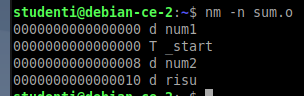
\includegraphics{img/141.PNG}
	\end{center}
	abbiamo le etichette utilizzate in \emph{.data} e in \emph{.text}.
	\item \begin{verbatim}ld -o sum sum.o\end{verbatim}
	collegatore, indico come argomenti i files oggetto da collegare. Viene generato il file eseguibile.
	\item \begin{verbatim}./sum\end{verbatim}
	indico il nome dell'eseguibile per eseguire il programma. In questo caso non viene mostrato nulla, visto che il programma effettua solo spostamenti di memoria.
	\item \begin{verbatim}objdump -d sum\end{verbatim}
	richiedo nuovamente il \emph{disassembly}. \begin{center}
		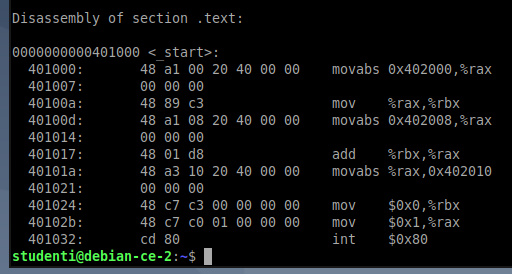
\includegraphics{img/142.PNG}
	\end{center}Otteniamo la stessa cosa di prima, ma vediamo che gli indirizzi dei dati sono definiti. Domanda che sorge spontanea: l'eseguibile è un file oggetto? Il file oggetto visto prima e l'eseguibile hanno lo stesso formato (\emph{file format elf64-x86-6}). 
	\begin{itemize}
		\item L'OPCODE occupa al più due byte.
		\item In presenza di indirizzi e costanti aumenta la dimensione dell'istruzione. Si ha minore occupazione di memoria coi registri.
		\item Attenzione al \emph{little-endian}.
	\end{itemize}
\end{itemize}


\paragraph{Ragioniamo sul programma}
\begin{itemize}
	\item Il programma ha lo scopo di sommare due numeri \emph{quad}. 
	\item Si osservino i passaggi che facciamo con l'istruzione \emph{movabs}, necessari per evitare probabili troncamenti dell'indirizzo a causa dell'\emph{offset} a 32 bit (spazio insufficiente per contenere l'intero indirizzo, se succede il programma inchioda e segnala errore). La cosa dipende da dove sarà collocato in memoria il nostro programma: non lo possiamo sapere a priori, dunque conviene prevenire. 
	\item La movabs viene eseguita più volte poichè l'unico registro destinatario possibile è RAX.
	\item Il collegatore vede solo le etichette .global 
	\begin{verbatim}
		.global _start
	\end{verbatim}In questo caso la utilizzo per dichiarare l'\emph{entry point} del mio programma.
	\item In .data inizializzo i byte che conterranno i miei dati.  
	\begin{verbatim}
		.data
		num1:
		.quad 0x1122334455667788
		num2:
		.quad 0x9900aabbccddeeff
		risu:
		.quad -1
	\end{verbatim}
	Possiamo inizializzare \emph{byte} (8 bit, 1 byte), \emph{word} (16 bit), \emph{long} (32 bit) e \emph{quad} (64 bit). Si consideri che le etichette non occupano spazio e ci permettono di dare nomi ad aree che vedranno associato un indirizzo solo dopo. 
	\item \textbf{Cosa succede se non definisco il valore iniziale dell'insieme di byte introdotto con la direttiva?} Non viene allocato lo spazio! 
	\item \textbf{Non è importante ottimizzare il programma}: non vogliamo diventare programmatori di Assembler. Il compilatore è molto più bravo di noi in questo.
	
	\item \textbf{Sintassi nuova a 64bit}. Riprendiamo la seguente cosa
	\begin{verbatim}
		num1(%rip)
	\end{verbatim}
	L'assemblatore prende questa cosa come l'ordine di calcolare l'offset tra num1 e rip, cioè la differenza. Questa "scappatoia" permette di risolvere il problema del troncamento dell'indirizzo per spazio insufficiente. Il disassemblatore, se abbiamo utilizzato il collegatore, ci restituisce l'indirizzo. Si osservi che in instruzioni diverse l'offset è diverso. Il fatto che non siamo noi a calcolare l'offset è sicuramente una semplificazione. Se riprendiamo gli esempi di indirizzamento di Reti logiche ci ricordiamo che in quei casi dobbiamo indicare noi lo scostamento. Nel caso spiegato ora no.
	
	\item \textbf{Accesso ad aree di memoria}. L'idea base è che io possa accedere esclusivamente alle cose che ho dichiarato. Questa cosa è assolutamente falsa: io posso scrivere dove mi pare, tenendo conto di alcuni limiti. Il kernel, se accediamo ad aree di memoria dove non abbiamo permessi, ci segnala errore di \emph{Segmentation Fault}. Osserviamo lo spazio allocato per il nostro programma: se io accedo a 402000 (dove c'è num1) non avrò problemi. Posso accedere senza problemi fino all'indirizzo 402ff0 (se eseguo un'operazione di MOV non ho problemi). Non appena mi sposto di un solo byte mi viene nuovamente segnalato segmentation fault.
	\item \textbf{Cosa succede se scrivo..?}
	\begin{verbatim}
		mov %rax, num1+16
	\end{verbatim}
	Scrivo su risu. Chi calcola questa espressione? L'assemblatore o il collegatore (in questo caso il collegatore, num1 non è conosciuto dall'assemblatore)! Abbiamo un'espressione costante.
	Si osservi che l'assemblatore sa fare solo espressioni semplici.
\end{itemize}



\subsection{Debugger} Utilizzeremo lo GNU debugger, che possiamo chiamare col seguente comando
\begin{verbatim}
	gdb sum
\end{verbatim}
dove \emph{sum} è il nome dell'eseguibile.
\begin{center}
	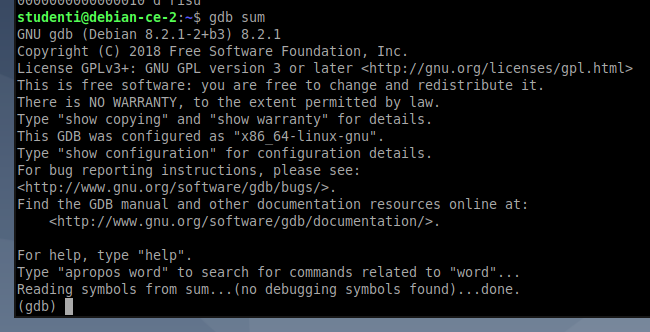
\includegraphics{img/143.PNG}
\end{center}
Il debugger è lo stesso visto a Reti logiche! Purtroppo è abbastanza spartano... Possiamo renderlo un po' più piacevole introducendo l'estensione \emph{gef} col seguente comando
\begin{verbatim}
	source ~/gef/gef.py
\end{verbatim}
Il programma non parte finchè non eseguiamo il comando \emph{start}. Il programma parte e subito si ferma, restituendo il controllo al debugger.
\begin{center}
	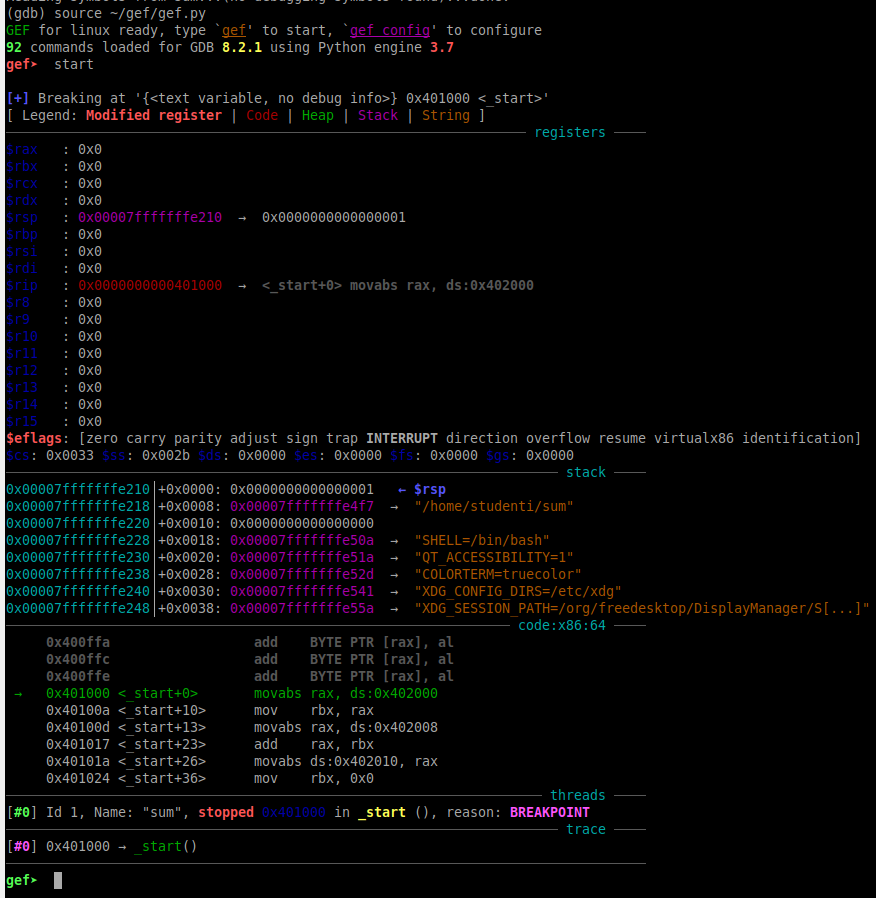
\includegraphics[scale=.9]{img/144.PNG}
\end{center}
L'estensione gef ci mostra, ogni volta che si ferma il debugger:
\begin{itemize}
	\item la lista dei registri con relativo contenuto (vengono evidenziati i registri che sono cambiati di valore rispetto alla "fermata" precedente);
	\item tra i registri quello dei flag (nomi dei flag, evidenziati se il valore è 1);
	\item la pila;
	\item il disassemblato.
\end{itemize}
Vediamo alcune azioni che potrebbero tornarci comode:
\begin{itemize}
	\item \textbf{Disassemblato in formato Intel}: il disassemblato di default (quello in foto) è in sintassi Intel, possiamo impostare la sintassi a cui siamo abituati con i seguenti due comandi
	\begin{verbatim}
		set disassembly-flavor att <----- imposto la sintassi a cui siamo abituati
		context <---- ricarico il contenuto
	\end{verbatim}
	\begin{center}
		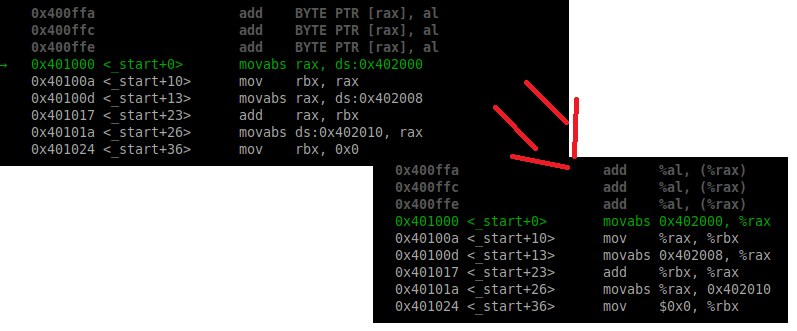
\includegraphics[scale=.9]{img/145.PNG}
	\end{center}
	\item \textbf{Configurazione dell'estensione gef}: il seguente comando
	\begin{verbatim}
		gef config
	\end{verbatim}
	mi permette di caricare la lista delle impostazioni dell'estensione gef.
	\begin{center}
		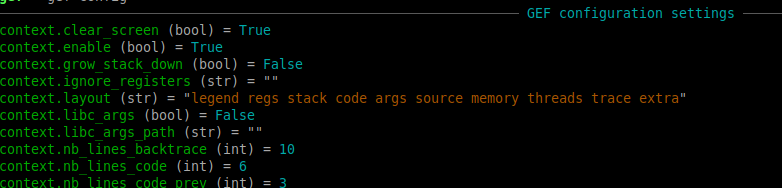
\includegraphics{img/146.PNG}
	\end{center}
	\item \textbf{Modifica di impostazioni dell'estensione gef}: modifichiamo un'impostazione, precisamente la context.layout che indica cosa deve apparirci ogni volta che eseguiamo la context
	\begin{verbatim}
		gef config context.layout "regs code memory"
		context
	\end{verbatim}
	in questo modo abbiamo rimosso la pila (visibile per default, per il momento non ci serve). Mostriamo solo registri, codice e memoria.
	\begin{center}
		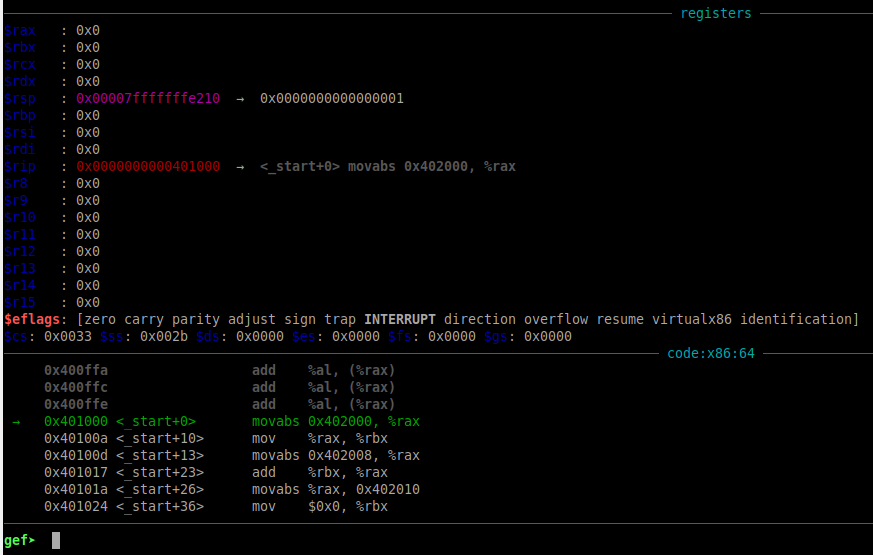
\includegraphics[scale=.9]{img/147.PNG}
	\end{center}
	\item \textbf{Contenuto della memoria a partire da un certo indirizzo nella schermata}: col seguente comando chiediamo di mostrare, a partire dall'indirizzo num1, tre qword
	\begin{verbatim}
		memory watch &num1 3 qword
		context
	\end{verbatim}
	\begin{center}
		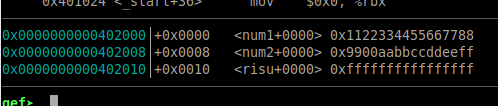
\includegraphics[scale=.9]{img/148.PNG}
	\end{center}
	\item \textbf{Esecuzione di una singola istruzione}: col seguente comando 
	il debugger cede il controllo al programma per eseguire una singola istruzione.
	\begin{verbatim}
		si
	\end{verbatim} 
	\item \textbf{Uscita dal debugger}. Ricordiamo il comando per uscire dal debugger
	\begin{verbatim}
		quit
	\end{verbatim}
\end{itemize}

\section{Indirizzi}
Abbiamo già detto che il processore lavora con indirizzi, e che ogni cosa deve essere identificata mediante un indirizzo.
\begin{itemize}
	\item \textbf{Prima cosa necessaria è avere dimestichezza con i numeri esadecimali}: sono comodi, una cifra esadecimale mi rappresenta quattro cifre binarie.
	%\item Certe volte servono anche i numeri ottali: una cifra ottale mi rappresenta tre cifre binarie. Le proprietà sono le stesse dei numeri esadecimali (l'unica differenza è il considerare terne invece di quaterne). La rappresentazione era utilizzata soprattutto in passato, quando i byte non esistevano ancora e i caratteri erano rappresentati su 6 bit.
	\item Gli indirizzi \emph{vanno pensati come circolari}: ripensare all'operatore modulo di Reti logiche.
	\[|11111111+00000001|_{2^8}=00000000\]
	\item Per rappresentare un indirizzo in C utilizziamo l'\emph{\textbf{unsigned long}}. Attenzione alle direttive:
	\begin{itemize}
		\item in caso di overflow di un \emph{unsigned long} ripartiamo da zero (cosa pensata proprio per gli indirizzi);
		\item in caso di overflow di un \emph{long} sostanzialmente \emph{fa quello che vuole}, si ottiene un \emph{undefined value}.
	\end{itemize}
	\item Il compilatore del C può assumere, per motivi di efficienza, che la condizione non accada mai. Prendiamo il seguente esempio
	\begin{verbatim}
		long x;
		if(x+1 < x)
		...
	\end{verbatim}
	il compilatore ignora completamente la condizione, visto che non sarà mai vera. \textbf{Non avverrà la stessa cosa in presenza di un \emph{unsigned long}}: in quel caso la condizione ha senso e permette di verificare se c'è stato overflow.
\end{itemize}
\subsection{\emph{Offset} (o scostamento)}
\begin{itemize}
	\item L'\emph{offset} consiste nella distanza tra due indirizzi $x$ ed $y$. 
	\item Lo scostamento, precisamente, rappresenta il numero di byte che dobbiamo saltare per passare dall'indirizzo $x$ all'indirizzo $y$. 
	\item La cosa vale con $x<y$, ma anche con $x>y$ (cioè l'offset può essere anche negativo). Vale anche quando abbiamo l'overflow, e quindi il modulo riparte da zero (circolarità dell'operatore modulo).
	\item \textbf{Attenzione} al dimensionamento dell'area dove poniamo l'offset. Se è inferiore alla dimensione degli indirizzi potrebbero emergere problemi.
\end{itemize}
\clearpage 

\subsection{Intervalli (\emph{range})} 
Un intervallo è una sequenza di indirizzi.
\paragraph{Convenzione}
Per convenzione gli intervalli presentano la seguente forma
\[[x,y)=\{z|x \leq z < y\}\,\,\,\,\,\,\,\,\text{con $x \geq y$}\]
Questo ci permette di combinare facilmente due intervalli consecutivi. Per semplicità evitiamo di considerare intervalli che attraversano l'ultimo indirizzo rappresentabile e ripartono da zero (che avrebbero $y<x$). L'insieme $[x,y)$ è vuoto se $y\leq x$.
\paragraph{Grandezza dell'intervallo} La grandezza dell'intervallo è esattamente $y-x$.
\paragraph{Base dell'intervallo} $x$ è detta \emph{base dell'intervallo}. Il suo indirizzo è l'indirizzo dell'intervallo.
\subsubsection{Divisione dello spazio di memoria in parti uguali}
Molto spesso conviene immaginare lo spazio di memoria diviso in parti uguali, ciascuna di dimensione di una potenza di due. 
I punti in cui si passa da un intervallo a un altro sono detti \emph{confini}. L'area compresa tra due confini non ha un nome in letteratura, noi la chiameremo \emph{regione naturale}.
Un indirizzo che si trova al confine si riconosce in maniera immediata:
\begin{center}
	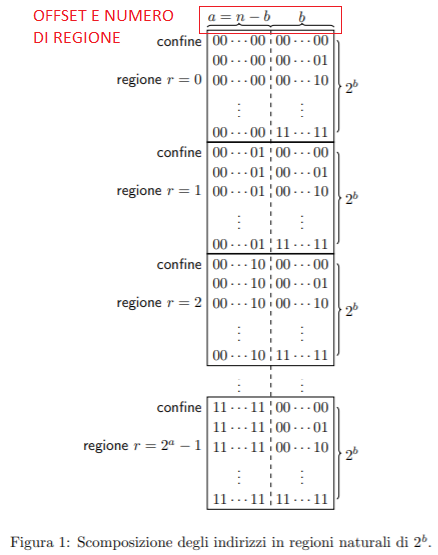
\includegraphics{img/6.PNG}
\end{center}
Osserviamo la struttura dell'indirizzo di base e la struttura dell'ultimo indirizzo di un intervallo. Dati $n$ bit di un indirizzo avrò:
\begin{itemize}
	\item i $b$ bit meno significativi come \textbf{offset} (precisamente l'offset rispetto all'indirizzo di base del relativo intervallo), e
	\item gli $n-b$ bit più significativi come \textbf{numero di regione}.
\end{itemize}
\begin{framed}
	\noindent \textbf{Come pongo questi numeri in due variabili C++?}
	\begin{verbatim}
		unsigned long x;
		
		unsigned long nr = x >> b;
		unsigned long off = x & ((1 << b) - 1);
	\end{verbatim}
	\begin{itemize}
		\item \textbf{Numero di regione}: traslo a destra $b$ volte. Non posso usare una maschera perché otterrei il numero di regione naturale moltiplicato per $2^b$.
		\item \textbf{offset}: utilizzo l'operatore AND e una maschera che mi lascia solo i $b$ bit meno significativi. L'operazione mi permette di ottenere $2^b-1$.
	\end{itemize}
\end{framed}
\paragraph{Intervallo che inizia in una regione e finisce in un'altra} Come trovo l'ultima regione toccata dall'intervallo $[x,y)$ ? 
\begin{itemize}
	\item Per prima cosa devo controllare che l'intervallo non sia vuoto, per esempio $[x,x)$, 
	\item se non lo è mi basta prendere il numero di regione di $y$.
\end{itemize}
\paragraph{perché ci servono queste spiegazioni?} Parleremo di memoria RAM e periferiche che occupano porzioni di indirizzi, appunto \emph{intervalli}. Lavoreremo (con una singola istruzione) su oggetti di un byte, due, quattro, otto byte.

\paragraph{Oggetto allineato in memoria} Un oggetto si dice \emph{allineato} a qualcosa se il suo indirizzo è multiplo di una qualche potenza di due, cioè se l'indirizzo si trova a confine di una qualche regione naturale. Vediamo delle espressioni frequenti:
\begin{itemize}
	\item Oggetto allineato a $2^b$
	\item Oggetto allineato a $Y$ (cioè un oggetto tale che $\dim Y = 2^b$)
	\item Oggetto allineato naturalmente (cioè l'oggetto è allineato alla sua dimensione, $\dim 2^b$).
\end{itemize}